\chapter[Integrationsprozesse]{Integrationsprozesse}

Nach den behandelten Herausforderungen werden in diesem Kapitel Möglichkeiten und Vorgehensmodelle zur Integration von Data Science in Organisationen thematisiert.
Dazu werden insgesamt drei Modelle der Forschungsliteratur dargelegt.

\section{CSPG Framework}

\Citeauthor*{Grossman.2014} veröffentlichte 2014 das CSPG Framework zur Integration von Analytik, Domänenwissen und IT in Organisationen.
\textit{CSPG} steht repräsentativ als Abkürzung für die Komponenten \textit{Culture, Staffing, Processes} und \textit{Governance}. 
Der Aspekt der Kultur ist durch die Organisationsleitung umzusetzen, indem Verantwortung und Autorität für Datenbestände an eine Funktionsstelle übergeben wird.
Die Aufnahme von Data Science Personal ist im CSPG Framework unausweichlich und durch den Analytik Leiter und die Geschäftsleitung durchzuführen. 
Dabei ist zu entscheiden, ob die analytische Funktion zentral, dezentral oder hybrid organisiert wird.
Im dritten Aspekt des Frameworks sind die analytischen Prozesse in der Organisation aufzubauen.
Ein Teil dieser Prozesse umfasst den Austausch von Daten zwischen Abteilungen und anderen Organisationen.
Weitere Prozesse behandeln die Digitalisierung bestehender Inhalte, Produktanpassung zur Aufnahme von Daten und die Kombination von Datenbeständen.
Die finale Komponente des Frameworks ist der Aufbau, die Verwaltung und die Weiterentwicklung der notwendigen Infrastruktur.
Zur Bewältigung dieser Aufgabe sind die folgenden vier Bedingungen in der Organisation zu erfüllen:

\begin{itemize}
    \item Langfristige Verpflichtung für Data Science und Sicherstellung des daraus entstehenden Geschäftswerts.
    \item Sichere und rechtlich unbedenkliche Umsetzung der Data Science Prozesse.
    \item Herstellen von Haftbarkeit, Transparenz und Rückverfolgbarkeit für Projektfinanzierung, Entwicklung und Ressourcen.
    \item Ressourcenbereitstellung für Daten-, Analyse- und Managementprozesse.
\end{itemize}

\section{Design Parameters}

Durch die Arbeit von \Citeauthor*{JanineAdinaHagen.2020} konnten die Gestaltungsparameter einer datengesteuerten Organisation ermittelt werden.
Diese Parameter können als Richtlinien betrachtet werden, wie die eigene Organisation in verschiedenen Aspekten zu gestalten ist.

\begin{figure}[htb]
    \centering
    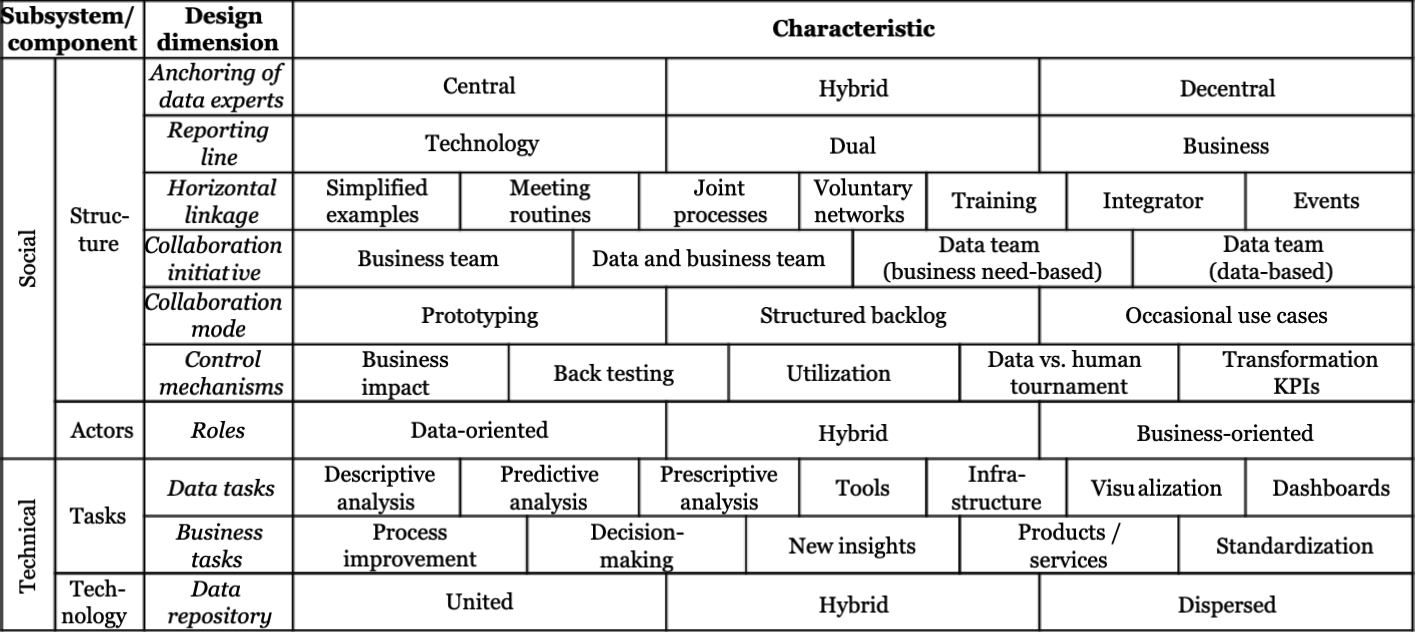
\includegraphics[width=0.75\textwidth]{graphics/DDO_design.png}
    \caption{Gestaltungsparameter einer datengesteuerten Organisation}
    \label{fig:DDOs design}
\end{figure}

Die vorherige Tabelle zeigt die Gestaltungsparameter organisiert nach Komponenten, Dimensionen und konkreter Charakteristika. \footcite[Vgl.][S. 5]{JanineAdinaHagen.2020}
Eine wichtige Komponente betrachtet die soziale Perspektive auf die Struktur und die Akteure der datengesteuerten Organisation.
Die Struktur der Organisation kann durch die Parameter \textit{Expertenorganisation, Berichtslinie, horizontale Verknüpfung, Kooperationsinitiative, Kooperationsmodus} und \textit{Kontrollmechanismus} beeinflusst werden.
Eine mögliche Ausprägung dieser Parameter umfasst z. B. zum einen dezentrale Data Science Experten, eine Berichtslinie zur Fachabteilung sowie regelmäßige Meetings und Events der Data Science Experten.
Zum anderen werden z. B. durch die Datenexperten die Zusammenarbeiten mittels strukturiertem Backlog initiiert und anhand des Geschäftsmehrwerts evaluiert.
In dieser Struktur könnten dann die Rollen z. B. hybrid, also datenorientiert sowie geschäftsorientiert gestaltet werden.
Wird die technische Perspektive betrachtet, werden dessen Komponenten der Aufgaben und Technologien durch die Parameter \textit{Datenaufgaben, Geschäftsaufgaben} und \textit{Datenrepository} bestimmt.
Beispielhaft könnte eine Organisation durch ihre Struktur und Akteure beschreibende, prädiktive und vorhersagende Analysen erstellen, um Prozesse zu verbessern und Entscheidungen zu unterstützen.
Speicherorte für Daten und Software können z. B. hybrid für jedes Datenteam einer Fachabteilung und für den gemeinsamen Austausch mehrerer Datenteams eingerichtet werden.

\section{Experiment Evolution Model}

Ein weiteres Vorgehensmodell durch \Citeauthor*[][]{Fabijan.2017} beschreibt den Transformationsprozess von Ad hoc Analysen zu skalierten kontrollierten Experimenten in Organisationen. \footcite[Vgl.][S. 5]{Fabijan.2017}
Das Experiment Evolution Modell verdeutlicht die Evolutionsphasen datengesteuerter Entwicklung in Unternehmen und Abteilungen.
Zur Anwendung des Modells sind Voraussetzungen zu erfüllen, welche folgend thematisiert werden.

Eine Anwendung setzt insoweit Fähigkeiten der Data Science voraus, sodass Produktstatistiken evaluiert werden können.
Die Fähigkeiten umfassen das Verständnis von Hypothesentests, Randomisierung, Stichprobengrößen und die Berechnung von Konfidenzintervallen. %\footcite[Vgl.][S. 6]{Fabijan.2017}
% Falls derartige Fähigkeiten nicht vorliegen, können Onlineressourcen die Weiterentwicklung der Mitarbeiter unterstützen.
Die Kombination dieser Fähigkeiten mit Domänenwissen ermöglicht die Generierung und Evaluation erster Produkthypothesen.
Als zweite Anforderung wird die Verfügbarkeit eines Zugangs zu Daten der Produktverwendung vorausgesetzt.
% Je nach Domäne können dabei komplizierte Fragestellungen hinsichtlich rechtlicher sowie technischer Herausforderungen aufkommen.

Die im Modell abgebildete Evolution erfolgt in den drei Dimensionen Technisch, Organisatorisch und Geschäftlich. 
Jede Dimension folgt den vier Phasen \textit{Krabbeln, Gehen, Rennen} und \textit{Fliegen}.
Zu Beginn der ersten Phase finden in der technischen Dimensionen der Aufbau von Logging-Systemen und erste manuelle produktspezifische Analysen von Data Science Teams statt.
Die Geschäftsdimension beinhaltet die Definition von unternehmensweiten Evaluationskriterien in Verbindung mit den langfristigen Geschäftszielen.
Während der Phase des \textit{Gehens} werden in der technischen Dimension Metriken entwickelt, anhand dessen Eventdaten aggregiert betrachtet werden können.
Diese Phase erzeugt den Bedarf einer übergreifenden Analyseplattform durch das Wachstum an Experimentarten und Anwendungen. 
In der Organisation bauen während dieser Phase Data Science Experten zunehmend Wissen zu einzelnen Produkten auf.
Ebenfalls werden Daten und Vorgehensweisen weitreichend geteilt.
Die Geschäftsdimension entwickelt sich durch Validierung bestehender und Entwicklung neuer Evaluationskriterien z. B. hinsichtlich der Datenqualität.
Zur Phase des \textit{Rennens} werden in der technischen Dimension Analyseplattformen skaliert und Experimente für mehrere Produktteams ausgeführt, um einen Fokus auf nahverwandte Metriken der Geschäftsziele zu setzen.
Organisatorisch übernehmen Produktteams volle Verantwortung und für ihre Ergebnisse, werden aber noch fachlich von Data Science Experten begleitet.
In der Geschäftsdimension werden bisherige Qualitäts- und Leistungskriterien verfeinert und kombiniert, um Ergebnisse zu Standardisieren und wenige klare Ziele zu fokussieren.
Die letzte Phase des \textit{Fliegens} fokussiert in der technischen Dimension die Standardisierung der Metrikentwicklung, Erweiterung der Plattformautomatisierung und Aufnahme von Daten zu jeder Produktänderung.
Die Evolution der Organisation umfasst zu diesem Zeitpunkt die autonome Durchführung von Analysen durch Produktteams und Entwicklung von Plattformen durch zentrale Data Science Teams.
In der Geschäftsdimension sind zu dieser Phase lediglich periodisch Änderungen an definierten Evaluationskriterien und deren Entwicklungsprozessen vorzunehmen.

Das Modell lässt sich zusammenfassend wie folgt in Abbildung 5.2 darstellen. \footcite[Vgl.][S. 6]{Fabijan.2017}
\begin{figure}[htb]
    \centering
    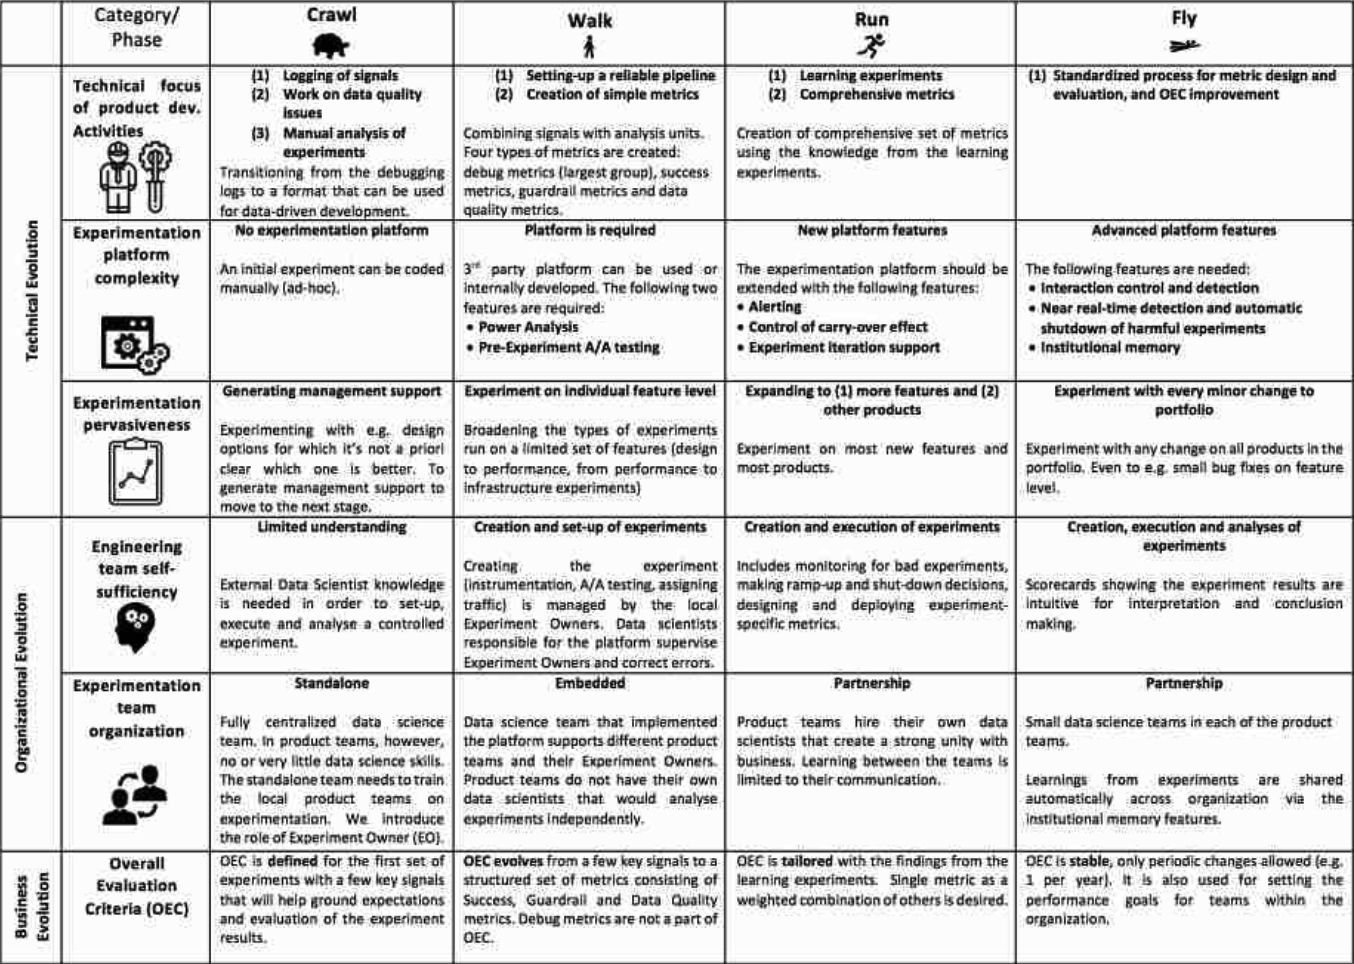
\includegraphics[width=0.67\textwidth]{graphics/EEM model.png}
    \caption{Gestaltungsparameter einer datengesteuerten Organisation}
    \label{fig:EEM model}
\end{figure}